\section{Workspace UI: documentation, profile and reliable feedback}
\label{workspace-ui}
\subsection{Problems addressed}
The previous pack list exposed technical IDs and review/trust strings as its main
content, with the Read action on another line. Lesson actions sent their messages
to an ordinary page toast outside a native modal dialog; that toast was behind the
browser's top layer and often inaccessible to the learner. XP appeared only in
Stats, while profile settings were mixed into More. There was no in-app guide.

The refreshed interface uses a restrained learning-workspace pattern: neutral
surfaces, a clear text hierarchy, compact lists, one accent for actions/current
position, and additional semantic colors only for results, milestones and errors.
Today keeps one primary next step, an optional shorter task, and a milestone when
one is relevant. The path is a consistent vertical sequence. Advanced controls
are disclosed when needed. The design has not been scored by an independent
professional designer and makes no claim about a measured motivational benefit.

\subsection{Reference review and adaptation}
The review inspected Duolingo's official learning-path redesign article, the HTB
Academy public SOC path, GitHub Primer's button documentation, Material Design's
list guidance, the WAI modal-dialog pattern, MDN top-layer documentation, and
Nielsen Norman Group's progressive-disclosure guidance. The register in
\path{docs/design/ui-workspace-sources.json} records URLs, access results and limits.
TryHackMe returned HTTP 429; no authenticated or access-restricted interface was
claimed as inspected. Duolingo's article is a historical design explanation, not
an audit of every current app screen.

The useful patterns are a guided next lesson, explicit prerequisites and course
structure, predictable primary/secondary/quiet actions, consistently placed list
actions, and help near the point of use. Primer's component states and Material's
scannable lists inform the controls. WAI guidance informs modal focus and Escape
behavior. Ascend retains its own content, brand and constraints; third-party
screenshots and brand assets are not shipped as product assets.

\subsection{Navigation and information hierarchy}
The persistent top bar shows the verified XP balance, day streak and a profile avatar. The
balance and streak open Stats; the avatar opens Profile. Actual server totals update after
verification and on refresh. No additional coin currency, invented rank or
spendable balance is introduced. An unavailable balance is shown as a dash rather
than a fabricated zero. Documentation can load without a successful account fetch.

Five primary destinations are Today, Path, Stats, Tracks and Docs. Profile is
reached through the top bar. Existing \texttt{\#more} links continue to resolve to
Tracks. The profile route is \texttt{\#profile}; documentation supports topic links
such as \texttt{\#docs/timers}. Profile contains identity, earned totals, timezone,
appearance, reminders and privacy. Tracks contains mission controls, the library
and saved ideas. A reader need not scan account settings to find an installed pack.

\subsection{Component and interaction contract}
\begin{longtable}{P{.22\textwidth}P{.70\textwidth}}
\textbf{Component} & \textbf{Behavior and rationale}\\\hline
Top bar & Persistent XP, day streak and avatar; clear accessible names and real server totals. Narrow layouts may shorten or hide the context label, preserving actions.\\
Track picker & Choose a domain first, then one of its installed tracks. Changing domains clears the track choice; starting requires a selected track and no active mission.\\
Library row & Human title, supporting counts/review state and a right-aligned Read button. The title and action share one row. A long title truncates visually but retains its accessible text and full preview.\\
Library controls & Search installed packs; initially show eight rows in a large library, with Show all/Show fewer. Import controls and parked ideas use disclosures.\\
Pack preview & Complete title and tasks grouped by level, with the first group open. Mark reviewed does not complete tasks or grant execution trust.\\
Lesson dialog & Fixed close/header and feedback regions surround an independently scrolling body. Initial focus goes to the title for a lesson and to the first field for the short logging form. Escape closes; focus returns to the opener.\\
Action feedback & The live region moves into the active dialog. Error and in-dialog messages persist until dismissed or replaced. Page-level informational messages last eight seconds. Timer reminders cannot replace an unresolved error.\\
Buttons & One filled primary action, outlined secondary actions and quiet text actions. Pending actions disable repeat submission and expose an accessible busy state; a small spinner provides feedback. Disabled and selected states remain distinct.\\
Docs & Ten searchable help topics with stable links, readable prose, working command-copy actions, and related guides. The guide can be read offline after the shell is installed; progress writes still require the server.\\
Profile & Actual account identity and verified totals, editable timezone, locally persisted theme, reminders and opt-in streak sharing. Unsupported username/password editing is not presented.\\
Path & Uniform vertical task rows, current-level emphasis and distinct ready, locked, done, skipped and milestone states. Color supplements labels and shapes.\\
Typography & Locally bundled Inter Variable with its SIL Open Font License. A limited hierarchy separates headings, body copy and supporting labels; mobile form text is 16 px to avoid focus zoom.\\
Motion & Short 140--180 ms transitions and a pending-action spinner. The next challenge has a 1.8-second glowing border sweep on its first visible display after each page load; tab changes and data refreshes do not replay it. Reduced-motion preference disables decorative animation and transitions.\\
\end{longtable}

The palette is defined once using CSS variables for light and dark themes. Light
mode uses background \texttt{\#f7f8fa}, text \texttt{\#242a38}, supporting text
\texttt{\#626b7a}, and accent \texttt{\#5147c7}. Dark mode uses background
\texttt{\#15181f}, text \texttt{\#eceef4}, and accent \texttt{\#b2aaff}.
Cards, fields and buttons use a small, consistent corner-radius and spacing scale.
The saved theme is applied before first paint. Fonts and the help guide are
bundled locally; no third-party font request is required during use.

\subsection{Implementation and evidence}
The account-scoped pack-list endpoint now includes title, kind, level count, task
count and validity. It still excludes private filesystem paths, user IDs and
fingerprints. Invalid private pack content does not prevent the rest of the library
from loading. Loading changed content rechecks its review/trust state before
returning metadata. There is no schema migration or progress rewrite for this UI.

The in-app guide is structured content in \path{web/guide.json}; the documentation
builder generates the matching LaTeX chapter from the same content. The service
worker caches that guide, the local font and theme bootstrap together with the
application shell. Private API responses remain uncached. The standalone wheel
regression checks the guide, font/license and theme asset and serves them from an
installed wheel outside the source checkout.

The expanded automated suite records 146 passing tests. Browser regressions cover
inline pack-row geometry, readable previews, in-dialog failure messages, persistence
of errors, Escape/focus restoration, XP updates after verification, profile/theme/
timezone persistence, guide search and direct links, and offline help. The visual
audit captures the actual browser at 320, 390, 768 and 1440 px, including dark mode.
Axe-core 4.10.3 checks WCAG 2 A/AA and 2.1 AA tagged rules on thirty screen/viewport
combinations. Its results are bounded automated evidence, not a claim of complete
accessibility conformance or an expert usability score.

After the final typography and documentation-focus adjustments, all fifteen
browser/integration regressions passed again. The \texttt{ascend:ui-workspace}
image built successfully and passed the shipped hardened Compose configuration:
read-only root filesystem, non-root user, bundled guide/font/theme assets, native
grading, signed receipt checks, and XP persistence across container restart. This
runtime check used AMD64 and disposable data; the previous ARM64 compatibility
evidence does not constitute a new physical Raspberry Pi run.

The existing local server was restarted with its original command and environment
after creating a SQLite backup in the private profile. Health and pack metadata
checks passed. Before/after comparisons confirmed unchanged mission, entry, node,
unlock, evidence, lab, timer and XP records. No demonstration progress was added
to the real profile.

Retained evidence is in \path{docs/testing/ui-workspace-tests.txt},
\path{docs/testing/ui-visual-audit.txt}, \path{docs/testing/ui-accessibility.json}
and \path{docs/screenshots/ui-workspace/}. Final browser, container and local-refresh
records are in \path{docs/testing/ui-final-regressions.txt},
\path{docs/testing/ui-deployment-smoke.txt} and
\path{docs/testing/ui-local-refresh.txt}. All screenshots and scored examples use
a disposable account; no real learner progress is manufactured for the demonstration.
A useful independent review is to try choosing a track, finding its requirements,
starting a lesson, recovering from a failed check, locating XP/profile settings and
finding help, using both keyboard and phone input.

\begin{figure}[htbp]
\centering
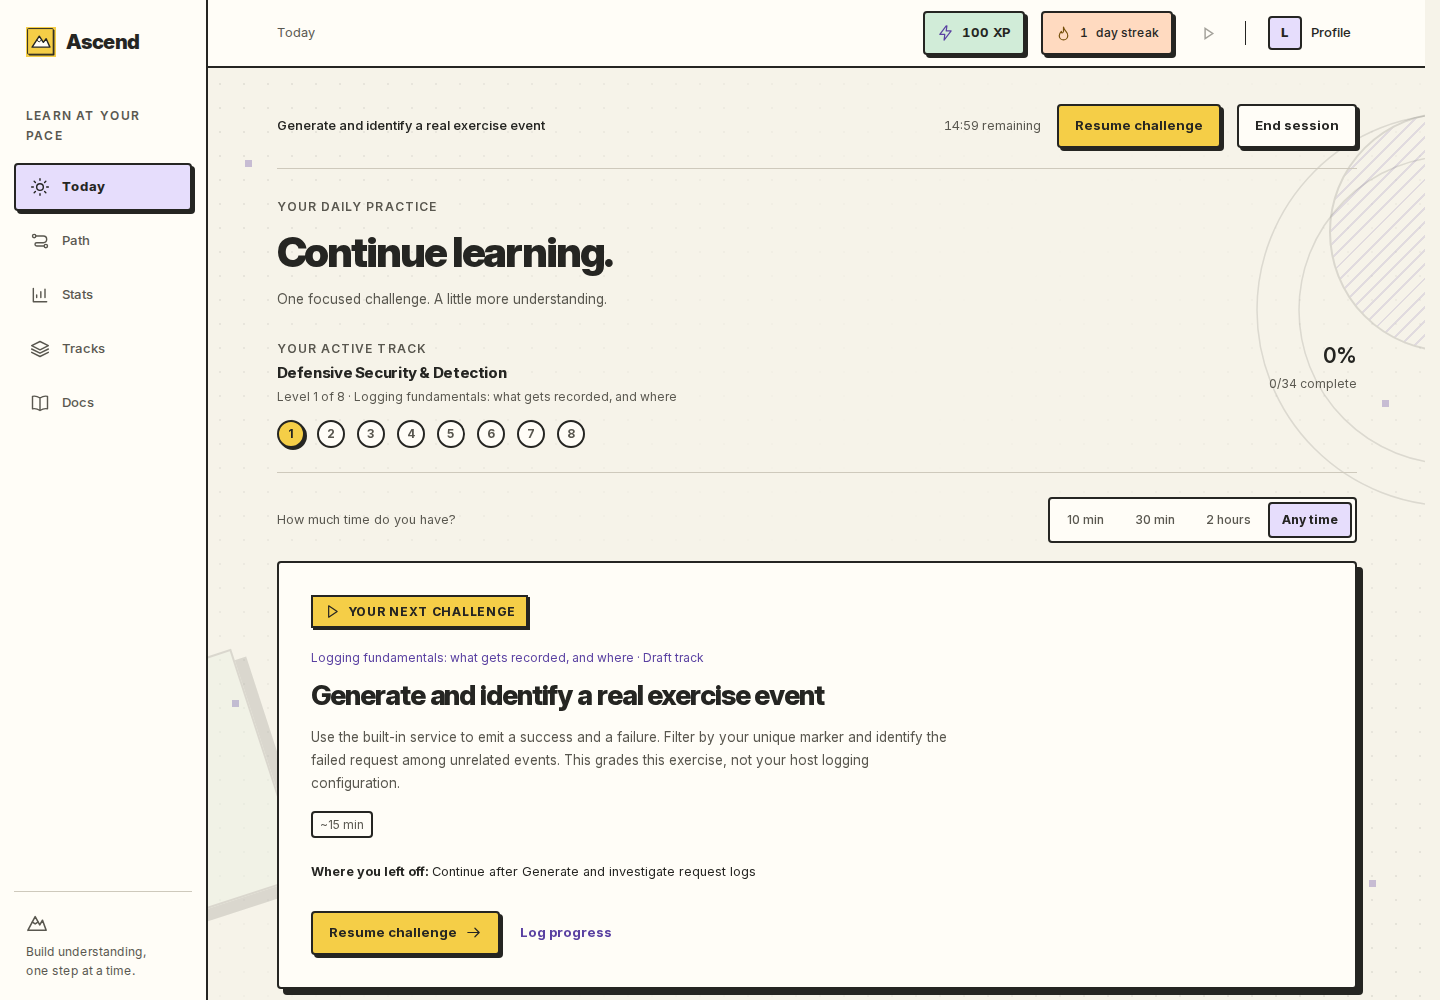
\includegraphics[width=\textwidth]{ui-workspace/today-desktop.png}
\caption{Current workspace: persistent XP/profile access, one primary learning action and restrained supporting content. Disposable demonstration account.}
\end{figure}
\begin{figure}[htbp]
\centering
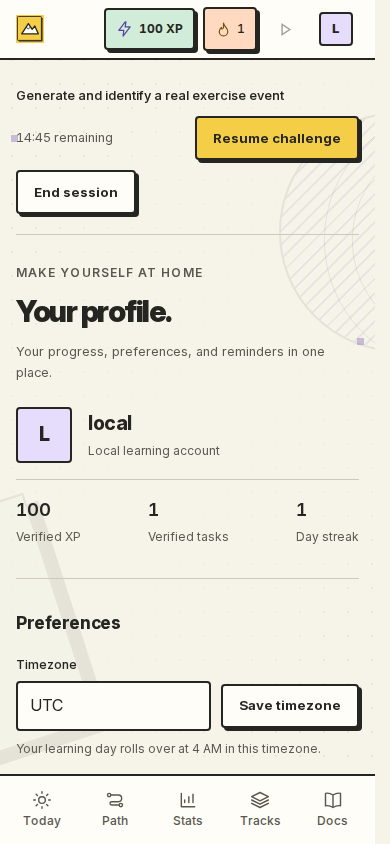
\includegraphics[width=.43\textwidth]{ui-workspace/profile-mobile.png}\hfill
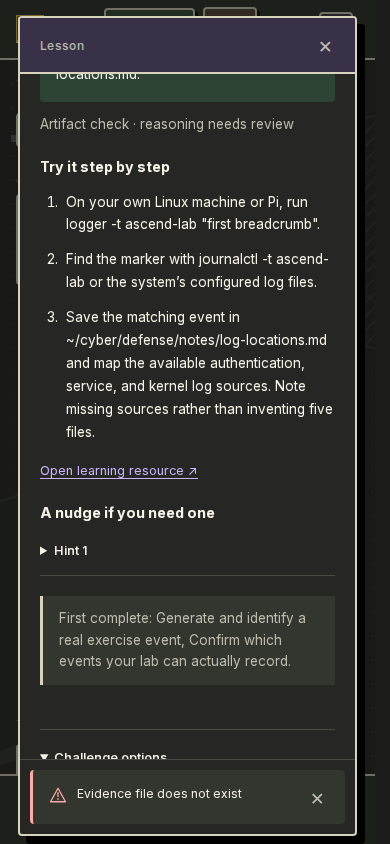
\includegraphics[width=.43\textwidth]{ui-workspace/lesson-feedback-mobile-dark.png}
\caption{Profile on mobile and visible feedback inside a dark-mode lesson dialog. These are viewport captures, not stitched page layouts.}
\end{figure}
